\documentclass[tikz,border=2mm]{standalone}
\usetikzlibrary{positioning, arrows.meta}
\begin{document}
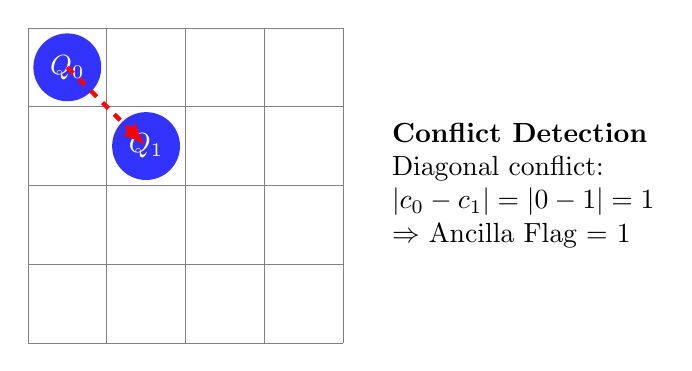
\begin{tikzpicture}[
    queen/.style={circle, fill=blue!80, text=white, minimum size=0.6cm, font=\bfseries}
]
\draw[step=1cm,gray,very thin] (0,0) grid (4,4);
\node at (0.5,3.5) [queen] {$Q_0$};
\node at (1.5,2.5) [queen] {$Q_1$};

\draw[red, ultra thick, dashed, -{Latex[length=3mm]}] (0.5,3.5) -- (1.5,2.5);

\node[anchor=west, align=left] at (4.5, 2) {
    \textbf{Conflict Detection}\\
    Diagonal conflict:\\
    $|c_0 - c_1| = |0 - 1| = 1$\\
    $\Rightarrow$ Ancilla Flag = 1
};
\end{tikzpicture}
\end{document}
